\section{Contribution}
\begin{itemize}
    \item []\textbf{113550002} 撰寫遞迴code、繪製內容圖片、製作書面報告、上台發表
    \item []\textbf{113550007} 撰寫dp、矩陣快速冪code、結論公式推導證明、上台發表
    \item []\textbf{113550018} 上影片字幕、上台發表
    \item []\textbf{113550159} code執行與生成結果、製作結果圖表、撰寫書面報告內容、上台發表
    \item []\textbf{113550179} 數據統整、製作影片、製作簡報、撰寫影片講稿、上台發表
\end{itemize}


\section{Rail}
\label{rail}
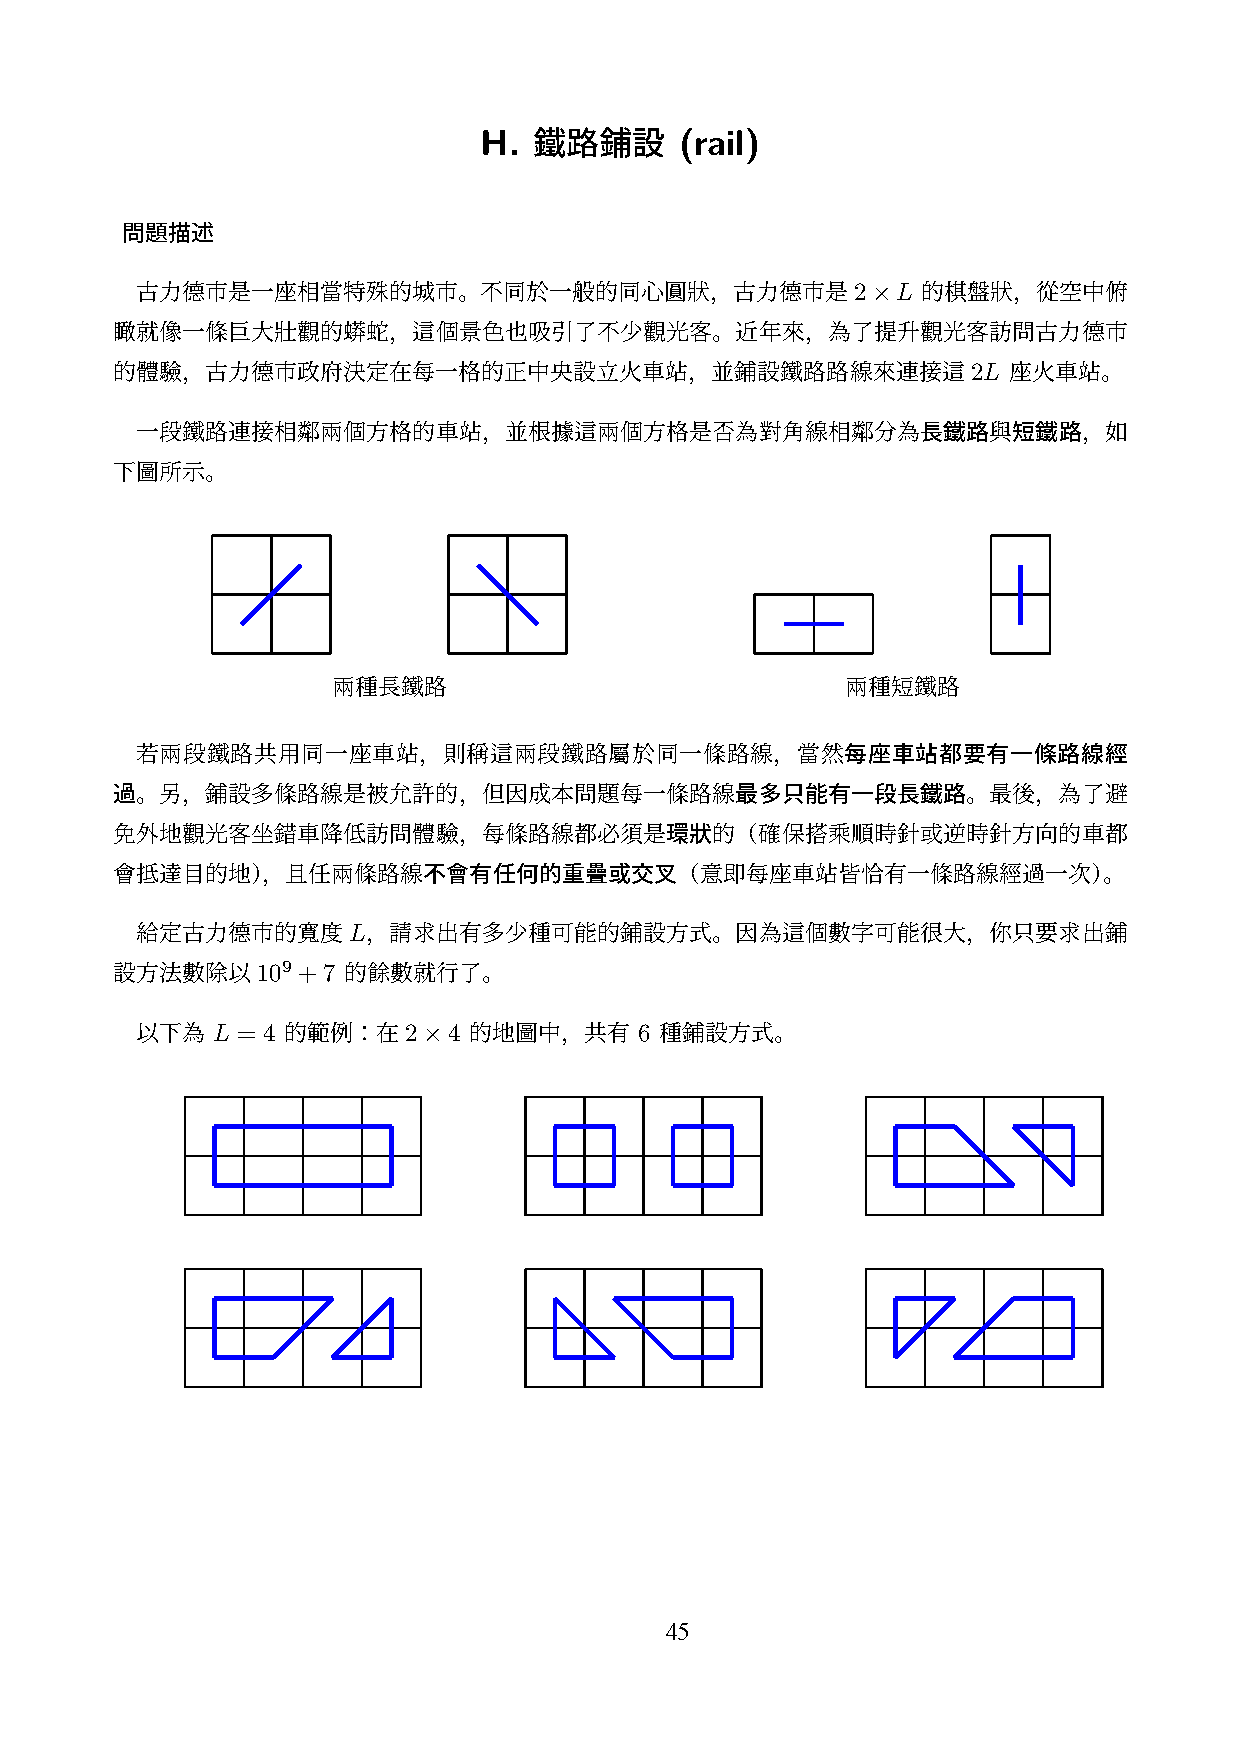
\includepdf[pages=-]{appendices/rail.pdf}

\section{Induction for the Transition Matrix of Rail}
\label{induction for Rail}

\subsection{Induction to recursive formula} 

\section{Code for Fibonacci}
\label{Fibonacci Code}
\subsection{Using Recursion}
\lstinputlisting[language=C++]{appendices/fibonacci_recursion.cpp}

\subsection{Using DP}
\lstinputlisting[language=C++]{appendices/fibonacci.cpp}

\subsection{Using Fast Matrix Power}
\lstinputlisting[language=C++]{appendices/fibonacci_bignum_2.cpp}

\section{Code for Rail}
\label{Rail Code}
\subsection{Using Recursion}
\lstinputlisting[language=C++]{appendices/rail_recursion.cpp}
\subsection{Using DP}
\lstinputlisting[language=C++]{appendices/rail.cpp}
\subsection{Using Fast Matrix Power}
\lstinputlisting[language=C++]{appendices/rail_bignum.cpp}